% $Author: ducasse $
% $Date: 2005/09/17 16:33:53 $
% $Revision: 1.1 $
\ifx\wholebook\relax\else
\documentclass{report}
\usepackage{times}
\usepackage{epsfig}
\usepackage{alltt}
\usepackage{xspace}
\usepackage{graphicx}
\usepackage{ifpdf}
\usepackage{ifthen}
\usepackage{amsmath}
\usepackage{a4wide}

\graphicspath{{figures/}} 

\ifpdf
\DeclareGraphicsExtensions{.pdf, .jpg, .tif, .png}
\else
\DeclareGraphicsExtensions{.eps, .jpg}
\fi

\newboolean{toseecomment}
\setboolean{toseecomment}{false}
%%change to false to hidde comment 
\newcommand{\comment}[1]{\ifthenelse{\boolean{toseecomment}}{$\blacktriangleright$ \textit{#1}$\blacktriangleleft$}{}}

\newcommand{\commented}[1]{}

\newboolean{seevwspecific}
\setboolean{seevwspecific}{true}
\newcommand{\vwspecific}[1]{\ifthenelse{\boolean{seevwspecific}}{#1}{}}

\newboolean{seecategoryspecific}
\setboolean{seecategoryspecific}{false}
\newcommand{\categoryspecific}[1]{\ifthenelse{\boolean{seecategoryspecific}}{#1}{}}

\newboolean{seestorespecific}
\setboolean{seestorespecific}{true}
\newcommand{\storespecific}[1]{\ifthenelse{\boolean{seestorespecific}}{#1}{}}

\newboolean{seesqueakspecific}
\setboolean{seesqueakspecific}{false}
\newcommand{\squeakspecific}[1]{\ifthenelse{\boolean{seesqueakspecific}}{#1}{}}


\newcommand{\category}[0]
{\ifthenelse{\boolean{seestorespecific}}
	{package\xspace}
	{category\xspace}}

\newcommand{\ct}[1]{\texttt{#1}\xspace}
\newcommand{\stc}[1]{{\small {\sf #1}}\xspace}
\newcommand{\ST}{{\textsc Smalltalk}\xspace}
\newcommand{\tab}{\makebox[4em]{}}
\newcommand{\ttt}[1]{{\tt #1}}
\newcommand{\chev}{\ttt{>>}}
\newcommand{\vw}{VisualWorks\xspace}
\newcommand{\sq}{Squeak\xspace}
\newcommand{\store}{Store\xspace}
\renewcommand{\chaptername}{Exercise}
\newcommand{\exercise}{\vspace{0.2cm}\noindent \textbf{Exercise:}\xspace}

\newsavebox{\fminibox}
\newlength{\fminilength}

% Fait un truc encadre
\newenvironment{fminipage}[1][\linewidth]
  {\setlength{\fminilength}{#1-2\fboxsep-2\fboxrule}
        \begin{lrbox}{\fminibox}\begin{minipage}{\fminilength}}
  { \end{minipage}\end{lrbox}\noindent\fbox{\usebox{\fminibox}}}

% Pareil mais pas encadre (a utiliser pour ne pas couper une fonction

\newenvironment{nminipage}[1][\linewidth]
  {\setlength{\fminilength}{#1}
        \begin{lrbox}{\fminibox}\begin{minipage}{\fminilength}}
  { \end{minipage}\end{lrbox}\noindent\mbox{\usebox{\fminibox}}}

% Un alltt encadre
\newenvironment{falltt}
  {\vspace*{0.3cm}\begin{fminipage}\begin{alltt}}
  {\end{alltt}\end{fminipage}\vspace*{0.3cm}}

% Un alltt pas encadre
\newenvironment{nalltt}
  {\vspace*{0.3cm}\begin{nminipage}\begin{alltt}}
  {\end{alltt}\end{nminipage}\vspace*{0.3cm}}

% Une fonction encadree
\newenvironment{ffonction}[1]
  {\begin{fonction}[#1]
        \begin{fminipage}
\begin{alltt}
\rule{\linewidth}{0.5pt}}
{\end{alltt}\end{fminipage}\end{fonction}}

\newenvironment{codeonepage}
  {\begin{nminipage}\vspace*{0.2cm}\hrule\vspace*{0.1cm}
\begin{alltt}}
  {\end{alltt} \vspace*{-0.2cm}\hrule \vspace*{0.2cm} \end{nminipage}}

\newenvironment{code}
  {\vspace*{0.1cm}\hrule\vspace*{-0.1cm}\begin{alltt}}
  {\end{alltt}\vspace*{-0.2cm}\hrule \vspace*{0.1cm}}


\begin{document}
\fi

\chapter{Set, Dictionary et Bag}

\mainauthor{Bernard Pottier  }
%\date{\today}
%version plus courte
\section{Collections non-ordonn\'ees}





Les \'el\'ements de ces collections ne sont pas rang\'es selon un
ordre pr\'edictible~:  on ne peut pas acc\'eder aux \'el\'ements
via une cl\'e externe, tel qu'un index, ou un ordre connu. 
Cette propri\'et\'e est li\'ee au m\'ecanisme
d'adressage dit {\sl associatif}, o\`u la position d'un \'el\'ement
dans la collection d\'epend de la valeur de cet \'el\'ement
et de l'historique des acc\`es
(voir les explications en section \ref{sec:hash}).

La hi\'erarchie de classes se pr\'esente de la mani\`ere suivante:

\begin{scode}
Object ()

    Collection ()
        Bag ('contents')
        Set ('tally')
            Dictionary ()
            IdentitySet ()

\end{scode}

\begin{itemize}
\item \ct{Set} : collection garantissant l'unicit\'e des \'el\'ements.
\item \ct{Dictionary} : acc\`es par une cl\'e, 
qui est en g\'en\'eral un objet d'une classe d\'etermin\'ee.
La cl\'e garantit l'unicit\'e.
\item \ct{Bag} : chaque  \'el\'ement a un compteur associ\'e,
\end{itemize}

Une premi\`ere utilisation de ces collections est la 
mise en {\oe}uvre d'algorithmes tr\`es simples reposant uniquement sur leurs
propri\'et\'es~:
 
 ~\\{\em Trouver tous les mots apparus dans un texte} 
 \begin{scode} 
 
\stBar bobyADit lesMotsDeBoby \stBar
bobyADit := 'ta pa ta pa tapa tout dit tapa tout dit a ta dou dou'.
lesMotsDeBoby := bobyADit tokensBasedOn: Character space.
lesMotsDeBoby asSet asSortedCollection asArray

 "#('a' 'dit' 'dou' 'pa' 'ta' 'tapa' 'tout')"
\end{scode}

\newpage

\section{Set}

\subsection{Cr\'eation}
Les ensembles sont des collections dynamiques, qui grandissent en fonction des
besoins. On cr\'ee de nouveaux ensembles par \ct{Set new}, ou, si on est
capable d'appr\'ecier correctement une taille idoine, par \ct{Set new: nElements}.
Si on connait d\'ej\`a les \'el\'ements, parce qu'ils sont rang\'es dans une
autre collection, alors on peut aussi instancier par \ct{Set withAll: une Collection}.

L'algorithme (hachage) qui sert \`a la mise en {\oe}uvre des ensembles a de bonnes
caract\'eristiques en temps de recherche d'un \'el\'ement.

\subsection{Acc\`es}

L'usage simple de Set peut \^etre r\'esum\'e de la mani\`ere suivante~:

\begin{itemize}
\item \ct{unSet add: unObjet},\\  \ct{unSet addAll: uneCollection},
ajout dans l'ensemble.
\item \ct{unSet includes: unObjet} vrai ou faux selon que \ct{unObjet}
soit pr\'esent ou absent.
\item \ct{unSet remove: unObjet} ou \\
\ct{unSet remove: un Objet ifAbsent: unBlocException. }

Dans le premier cas, on enl\`eve \ct{unObjet} de \ct{unSet}, si cet objet
existe. Sinon, on d\'eclenche une erreur.

Si le programmeur n'est pas certain de la pr\'esence de l'objet cherch\'e,
il utilise la seconde forme en passant un bloc d'exception, qui peut
\^etre vide\ldots 

\item  \ct{unSet size} ~: nombre d'\'el\'ements pr\'esents dans l'ensemble,
\item  \ct{unSet capacity} ~: capacit\'e de stockage de l'ensemble.
Plus le rapport $ capacity / size $ est grand, plus le temps d'acc\`es risque d'\^etre
rapide.
\end{itemize}


\section{Dictionary}

Un Dictionnaire est un ensemble dont les \'el\'ements sont des instances
de la classe \ct{Association}, couplant une cl\'e (\ct{key}), et une valeur
(\ct{value}). L'unicit\'e d'une association dans un ensemble donn\'e est garantie
par l'unicit\'e de la cl\'e, propri\'et\'e h\'erit\'ee de la classe \ct{Set}.

Les instances de Association sont fr\'equemment cr\'e\'ees \`a l'aide du message
binaire \assoc. Par exemple, \ct{\#boulesRouges\assoc40} associe l'entier 40
au symbole \ct{\#boulesRouges}.

La structure de donn\'ees de dictionnaire implant\'ee par la classe \ct{Dictionary} est int\'eressante \`a plusieurs titres:

\begin{itemize}
\item Possibilit\'e de d\'esigner un objet par une cl\'e souvent symbolique
(Symbol, String, nombres\ldots)
\item Rapidit\'e d'acc\`es, due au hachage (m\^emes performances que
les ensembles, voir en  section \ref{sec:perf}).
\item Possibilit\'e d'utiliser les dictionnaires comme des tables de hachage,
et pour des cl\'es tout \`a fait quelconques.
\item Dynamicit\'e de la collection qui grandit avec les besoins.
\end{itemize}

\subsection { Cr\'eation et propri\'et\'es h\'erit\'ees de Set}

On peut se reporter \`a la description donn\'ee dans \ct{Set}. Si on souhaite utiliser \ct{Dictionary withAll: uneCollection}, il faut cependant retenir que tous les \'el\'ements de \ct{uneCollection} doivent \^etre des instances de la classe \ct{Association}. L'exemple qui suit montre comment ajouter un dictionnaire \`a un autre, comment cr\'eer un dictionnaire initialis\'e.

La cl\'e servant \`a adresser le dictionnaire est simplement un entier, la valeur est un caract\`ere extrait d'une chaine. On remplit le premier dictionnaire en notant les index des blancs et les index des ponctuations. Le dictionnaire apparait alors comme un tableau ``creux''.

\begin{scode}
testDico1
    "self testDico1"

    \stBar dico1 dico2 vers \stBar
    dico1 := Dictionary new.
    dico2 := Dictionary new. 
    vers := 'le petit homme de la jeunesse, a casse son lacet de soulier,'.
    vers keysAndValuesDo:
               [:index :car \stBar car = $  
                                            ifTrue: [ dico1 at: index put: car ] 
                                            ifFalse: [ car isLetter ifFalse: [ dico1 at: index put: car ]]].
   dico1 addAll: dico2 associations. "ajout d'un dictionnaire a un autre dictionnaire"
   ^Dictionary withAll: dico1 associations "creation d'un dictionnaire pre-rempli"
\end{scode}

Parmi les messages h\'erit\'es de la classe \ct{Set}, se trouvent les op\'erations ensemblistes qui portent sur les cl\'es: intersection, union, soustraction\ldots 
Dans le code ci-dessus, la soustraction des deux dictionnaires serait simplement
sp\'ecifi\'ee par \ct{dico1 - dico2}.

\subsection{Acc\`es, ajouts et  suppressions}

Les m\'ethodes les plus simples pour ins\'erer, supprimer, tester sont les suivantes~:

\begin{itemize} 
\item \ct{unDictionnaire at: uneCle put: unObjet},\\
par exemple \ct{dico at: \#titi put: 12}.

\item \ct{unDictionnaire add: uneAssociation},\\
par exemple \ct{dico add: \#titi\assoc12}.

\item \ct{unDictionnaire removeKey: uneCle},\\
par exemple \ct{dico removeKey: \#titi}. Le r\'esultat est la valeur associ\'ee \`a la cl\'e (12).

On dispose aussi de la variante  \ct{unDictionnaire removeKey: uneCle ifAbsent: unBloc}.

\item \ct{unDictionnaire includesKey: uneCle},\\
par exemple \ct{dico includesKey: \#titi} rendrait \ct{true} dans le contexte ci-dessus.

\item \ct{unDictionnaire includes: unObjet},\\
par exemple \ct{dico includes: 12} rendrait \ct{true}, alors que
\ct{dico includes: \#titi} rendrait \ct{false}, 

De m\^eme  \ct{unDictionnaire occurencesOf: unObjet}, rend le nombre de fois
o\`u \ct{unObjet} est apparu en valeur de l'association.
\item \ct{unDictionnaire keyAtValue: unObjet} renvoie une cl\'e associ\'ee
\`a une valeur, si toutefois cette valeur existe.
 par exemple \ct{dico keyAtValue: 12} rendrait \ct{\#titi}\ldots
\end{itemize}

\subsection{It\'erations}
On peut distinguer les it\'erations g\'en\'erales, portant sur les \emph{valeurs}
plut\^ot que sur les cl\'es, les it\'erations portant sur les cl\'es, et enfin 
celles qui portent sur le couple cl\'e-valeur.

\begin{itemize}
\item \ct{unDico do: unBloc}\\
it\'eration sur toutes les valeurs, par exemple:
\begin{scode}
   \stBar dicoDesMots versDePrevert stream \stBar
   dicoDesMots := Dictionary new.
   stream := WriteStream on: ''.
   versDePrevert := 'le petit homme qui dansait dans ma tete'.
   (versDePrevert tokensBasedOn: $ )
         do: [ :mot \stBar dicoDesMots at: mot asSymbol put: mot size ].
   dicoDesMots do: [:longueurs \stBar stream nextPutAll: longueurs printString; space].
   ^stream contents 
     " '2 4 4 5 7 3 2 5 '"
\end{scode}

La transformation de la chaine de caract\`ere en symbole (\ct{asSymbol}) 
n'est pas indispensable.

\item \ct{keysDo:} it\`ere sur les cl\'es du dictionnaires:

\begin{scode}
   ...
   dicoDesMots keysDo: [ :mot \stBar stream nextPutAll: mot; space ].
   ^stream contents
" 'dans tete homme dansait qui ma petit le '"

\end{scode}
\item \ct{keysAndValuesDo:} permet d'acc\'eder simultan\'ement \`a la cl\'e et \`a la valeur:

\begin{scode}
...
dicoDesMots keysAndValuesDo: [:mot :taille \stBar 
              stream nextPutAll: mot, '(', taille printString,')'; space].
..
" 'tete(4) homme(5) ma(2) petit(5) qui(3) le(2) dans(4) dansait(7) '"
\end{scode}

\item \ct{collect:} et   fonctionne sur les valeurs associ\'ees
aux cl\'es.
\begin{scode}
    \stBar dicoDesMots versDePrevert  \stBar
    dicoDesMots := Dictionary new.
    versDePrevert := 'les sept eclats de glace de ton rire etoile'.
    (versDePrevert tokensBasedOn: $ )
        do: [ :mot \stBar dicoDesMots at: mot size put: mot asSymbol ].
    ^ dicoDesMots collect:  [ :mot   \stBar mot reverse ]"
" OrderedCollection ('ed' 'not' 'erir' 'ecalg' 'eliote')"\end{scode}

\item \ct{select: unBloc}, \ct{reject: unBloc} op\`erent sur les valeurs associ\'ees
aux cl\'es, mais renvoient un dictionnaire.
\begin{scode}
...
    ^ dicoDesMots select:  [:mot   \stBar mot size <= 4 ]  
      " Dictionary (2\assoc#de 3\assoc#ton 4\assoc#rire )"
\end{scode}
\end{itemize}

\section{Bag}

Cette classe s'appuie sur \ct{Dictionary} ou \ct{IdentityDictionary} pour compter
le nombre d'occurences d'un \'el\'ement. L'int\'er\^et est triple: 
vitesse d'acc\`es (due aux dictionnaires), comptage, et compacit\'e
de la structure de donn\'ees si le nombre des occurrences est \'elev\'e.
\subsection{Ajouts et suppressions}

Les sacs (classe \ct{Bag}) ont un interface permettant d'ajouter ou d'enlever des
\'el\'ements:

\begin{itemize}
\item \ct{unSac add: unObjet}\\
Le compteur des occurences de \ct{unObjet} est incr\'ement\'e.

\item \ct{unSac remove: unObjet}\\
\ct{unSac remove: unObjet  ifAbsent: aBlock}\\
Le compteur des occurences de \ct{unObjet} est d\'ecr\'ement\'e.
Si ce compteur tombe \`a 0, l'objet disparait du sac.

Dans la seconde version le bloc d'exception est \'evalu\'e au cas o\`u l'objet
n'existe pas: enlever un objet absent est une erreur.

\item \ct{unSac addAll: uneCollection} ~~~~~ 
\ct{unSac removeAll: uneCollection}\\
ajoute ou enl\`eve une collection d'objets.
\item \ct{unSac add: newObject withOccurrences: n }\\
\ct{unSac removeAllOccurrencesOf: anObject ifAbsent: aBlock}\\
ajoute n occurences du m\^eme objet, ou enl\`eve toutes les occurences d'un objet.
\end{itemize}

\subsection{\'Enum\'erations}

\begin{itemize}

\item \ct{do: collect: inject: \ldots}~:
Le principe utilis\'e est d'\'evaluer les blocs param\^etres pour chaque \'el\'ement
de l'ensemble. Par exemple, si \ct{unObjet} apparait 10 fois dans le sac, il
y aura 10 \'evaluations du bloc param\^etre.

Lorsque l'it\'erateur renvoie une collection, celle-ci est \'egalement un \ct{Bag}.
Dans l'exemple qui suit \ct{voyelles} est un \ct{Bag} qui ne comporte que 
\ct{false} et \ct{true}.

{\em Compter les voyelles dans une chaine}
\begin{scode}
\stBar b voyelles \stBar
    b := Bag new.
    b addAll: 'il pleut sans cesse sur Brest'.
    voyelles := (b collect: [:lettre \stBar lettre isVowel ]).
    voyelles occurrencesOf: true 
    "8"
\end{scode}

\item \ct{valuesAndCountsDo: unBloc}~: S'il est utile d'associer les \'el\'ements
et leurs compteurs associ\'es, on utilise ce message et on construit un bloc
\`a deux param\^etres (\'el\'ement et son compteur).


\end{itemize}
~\\{\em Imprimer par ordre croissant le nombre de caract\`eres apparus dans une chaine}
\begin{scode}

\stBar stream sort \stBar
stream := WriteStream on: (String new:200).
"preparation d'une collection comportant des Associations triees selon le champs value"
sort := SortedCollection new sortBlock: [:a1 :a2 \stBar a1 value \texttt{<} a2 value].
'le petit homme qui chantait sans cesse' asBag valuesAndCountsDo: [:v :c \stBar sort add: v\assoc{} c].
sort do: [:association \stBar stream nextPut: association key ; space.
     stream nextPutAll: association value printString, ' - '].
     stream contents 
"'q 1 - p 1 - o 1 - l 1 - u 1 - n 2 - m 2 - h 2 - c 2 - 
  i 3 - a 3 - t 4 - s 4 - e 5 -   6 - '"
\end{scode}




%\section{Performances}
% \label{sec:perf}
%{\em On veut comparer les performances en insertion et suppression sur les collections
%\ct{Set}, \ct{SortedCollection} et \ct{OrderedCollection}. Dans un premier temps, on laisse l'ensemble grossir au fur et \`a mesure des besoins, en testant les 3 collections.
%Dans un second temps,  on fixe d'embl\'ee la taille de l'ensemble \`a 4 fois
%la taille des \'el\'ements. Dans les deux cas les objets ins\'er\'es sont des nombres r\'eels al\'eatoires. }

% \begin{itemize}
% \item \ct{Set new}\\
% Le programme affiche une taile de d\'epart \'egale \`a 3, une taille finale \'egale \`a 1361.
% Un relev\'e des temps d'insertion donne  des valeurs de 3739, 3494, 3059, 4338, 3536,
% alors que les temps de suppression sont~: 8287, 7332, 8216, 8058, 8250. Donc,
% le cout de la suppression est deux fois plus \'elev\'e dans ces circonstances...
% 
% \item \ct{Set new:8000}\\
% La taille de d\'epart et la taille d'arriv\'ee (apr\`es les ajouts) est la m\^eme: 8689.
% Voila un bref \'echantillon des temps d'insertion et de suppression:
% ajout, 2150, 1931, 1883; suppression, 2804, 2754, 2364.
% 
% Ici la suppression est \`a peine plus co\^uteuse que l'insertion.
% 
% 
% \end{itemize}

%\subsection{Boucle externe du test et formatage}
%On y reconnait un \ct{stream} en \'ecriture sur une chaine de caract\`eres,
%qui sera utilis\'e pour produire une table au format LaTeX (voir la table \ref{tab:perf}).

%Le bloc \ct{eval} poss\`ede deux param\^etres, l'un contient la classe sur laquelle
%on effectue le test de performance, l'autre est un bloc servant \`a instancier cette
%classe. On rep\`ere les 6 \'evaluations de ce bloc en fin de m\'ethode.

%Dans le bloc, le temps de calcul insertion/suppression est produit en exp\'ediant le
%message \ct{testCollection: aClass creationBlock: aBlock times: nTimes}. Ce message est d\'ecrit plus bas. 

%Il faut noter que l'on r\'ep\`ete \ct{nTimes} fois les op\'erations et que les
%temps sont rendus dans une \ct{OrderedCollection} de taille \ct{nTimes}.

%\begin{scode}
%testNew
%   "Test testNew"

%   \stBar stream eval resultats nTimes \stBar
%   nTimes := 3.
%   stream := WriteStream on: ''.
%   stream nextPutAll: 'Classe \& '.
%   nTimes timesRepeat: [stream nextPutAll: 'add', ' \& ', 'remove', '\& '].
%   stream nextPutAll: 'add moy.', ' & ', 'remove moy. ', '\verb=\\\hline='; cr.
%   eval := 
%         [ :aClass :aBlock \stBar 
%         \stBar sumX sumY \stBar
%         stream nextPutAll: aClass name, ' \& '.
%         resultats := self
%                  testCollection: aClass
%                  creationBlock: aBlock
%                  times: nTimes.
%         sumX := sumY := 0.
%         resultats
%            do: 
%               [ :point \stBar 
%               stream nextPutAll: point x printString, ' \& ', point y printString, ' \& '.
%               sumX := sumX + point x.
%               sumY := sumY + point y ].
%         stream nextPutAll: (sumX // resultats size) printString, ' \& ', 
%                            (sumY // resultats size) printString, '\verb=\\\hline='; cr ].
%   eval value: Set value: [ Set new ].
%   eval value: SortedCollection value: [ SortedCollection new ].
%   eval value: OrderedCollection value: [ OrderedCollection new ].
%   eval value: Set value: [ Set new: 8000 ].
%   eval value: SortedCollection value: [ SortedCollection new: 8000 ].
%   eval value: OrderedCollection value: [ OrderedCollection new: 8000 ].
%   ^stream contents
%\end{scode}

%
%\subsection{Boucle interne du test}
%{\em Ici, on effectue une s\'erie de mesures identiques sur une classe
%pass\'ee en param\^etre, que l'on instancie via un bloc \'egalement pass\'e 
%en param\^etre.

%\ct{tRand} est le temps de g\'en\'eration de 2000 nombres. \ct{tAdd} est le temps d'insertion, \ct{tRemove}, le temps de suppression.

%Le temps est \'evalu\'e en millisecondes en utilisant le message \ct{Time millisecondsToRun: unBloc}. On renvoie une collection de points comportant en abcisse le temps d'insertion, en ordonn\'ee le temps de suppression (par pure commodit\'e).}

%\begin{scode}
%testCollection: collClass creationBlock: aBlock times: n 
%   \stBar rand set2 tAdd tRemove tRand set1 resultats \stBar
%   resultats := OrderedCollection new: n.
%   rand := Random new. "Generateur de nombre aleatoire"
%   n
%      timesRepeat: 
%         [ set2 := aBlock value.
%         tRand := Time millisecondsToRun: [2000 timesRepeat: [rand next * 100]].
%         tAdd := Time millisecondsToRun: [2000 timesRepeat: [set2 add: rand next * 100]].
%         set1 := set2 copy asArray.
%         tRemove := Time millisecondsToRun: [set1 do: [:elt \stBar set2 remove: elt]].
%         resultats add: tAdd - tRand @ tRemove].
%   ^resultats
%\end{scode}

%\subsection{Bilan}

%\begin{table}[htb]
%\begin{center}
%\begin{tabular}{|l|l|l|l|l|l|l|l|l|}\hline
%Classe & add & remove& add & remove& add & remove& add moy. & remove moy. \\\hline\hline
%Set & 514 & 946 & 503 & 908 & 507 & 920 & 508 & 924\\\hline
%SortedCollection & 769 & 2983 & 805 & 1564 & 759 & 2787 & 777 & 2444\\\hline
%OrderedCollection & 50 & 1574 & 41 & 2876 & 17 & 1568 & 36 & 2006\\\hline\hline
%Set & 267 & 361 & 244 & 353 & 264 & 349 & 258 & 354\\\hline
%SortedCollection & 1380 & 2869 & 852 & 1551 & 1326 & 2846 & 1186 & 2422\\\hline
%OrderedCollection & 49 & 1544 & 5 & 2887 & 53 & 1613 & 35 & 2014\\\hline
%\end{tabular}
%\caption{Performances compar\'ees. Le premier groupe de tests porte sur des
%collections cr\'e\'ees avec \ct{new}. Le second groupe porte sur
%des ensembles port\'es, d'embl\'ee \`a une capacit\'e de 8000 }
%\label{tab:perf}
%\end{center}
%\end{table}

%\begin{itemize}
%\item On peut constater que le co\^ut du sous dimensionnement de la structure du d\'epart peut \^etre important : dans le cas de Set, cela compte pour un facteur 2.
%\item Si la structure est grande, le co\^ut en suppression est r\'eduit (le second Set
%est 4 fois trop grand, et on remarque que les suppressions sont \`a peine plus lentes
%que les insertions). Dans le cas contraire, le co\^ut des suppressions peut \^etre jusque
%deux fois plus \'elev\'e que celui des insertions.

%L'explication se trouve dans la gestion des collisions et le nombre de celles-ci\ldots

%\item l'acc\`es en insertion sur les \ct{OrderedCollection} est tr\`es rapide, 
%on ne peut pas en dire autant des suppressions.
%\item les \ct{SortedCollection} marquent un avantage en recherche qui n'apparait pas ici.
%\end{itemize}
 

%\section{D\'ecomposition d'un nombre entier en facteurs premiers}

%{\em D\'ecrire un algorithme de d\'ecomposition  s'appuyant sur un ensemble
%de diviseurs possibles. L'ensemble de ces diviseurs est r\'eduit chaque fois
%qu'un de ses \'el\'ements est trait\'e. S'il s'agit d'un diviseur, on
%r\'eduit les nombres de l'ensemble \`a l'aide de ce diviseur. Dans le cas
%contraire on \'elimine tous les multiples du diviseur. Les diviseurs
%sont accumul\'es dans un \ct{Bag}.}

%\begin{scode}
%!Integer methodsFor: 'set-exemple'!
%decompose
%   \stBar diviseurs diviseursPossibles nb minBlock min maxBlock max sizeColl \stBar
%   diviseurs := Bag new.
%   diviseurs add: 1. nb := self.
%   sizeColl := OrderedCollection new.
%   diviseursPossibles := (2 to: self // 2) asSet.
%   min := 2. max := 1.
%   minBlock := [:number \stBar min := min min: number].
%   maxBlock := [:number \stBar max := max max: number].
%   [diviseursPossibles isEmpty or: [nb = 1]]
%      whileFalse: 
%         [\stBar diviseur division \stBar
%         sizeColl add: diviseursPossibles size.
%         diviseur := min.
%         division := nb / diviseur.
%         min := nb // max.
%         (division isKindOf: Integer)
%            ifTrue: 
%               [diviseurs add: diviseur.
%               maxBlock value: diviseur.
%               minBlock value: diviseur.
%               nb := division.
%               diviseursPossibles := diviseursPossibles
%                        collect: 
%                           [:n \stBar 
%                           \stBar x \stBar x := n / diviseur.
%                           x := (x isKindOf: Integer)    ifTrue: [x]    ifFalse: [n].
%                           x \texttt{>} (nb / max)
%                              ifTrue: [x := min]
%                              ifFalse: [(#(0 1) includes: x) ifTrue: [x := max]].
%                           minBlock value: x.
%                           x]]
%            ifFalse: [diviseursPossibles := diviseursPossibles
%                        reject: 
%                           [:n \stBar  minBlock value: n.
%                           ((n / diviseur isKindOf: Integer) or: [n \texttt{>} (nb / max)])
%                              or: [n = diviseur]]]].
%   Transcript cr; show: sizeColl printString ; cr.
%   ^diviseurs
%"(3*25*8*10*4) decompose  
% OrderedCollection (11999 5999 2999 1499 749 374 186 93 93 20 13 13 1 1)
% Bag (1 2 2 2 2 2 2 3 5 5 5)"
%\end{scode}

%\section{Hachage}
%\label{sec:hash}

%Le hachage d'un objet permet d'adresser une table par le contenu.
%Cette technique permet d'\'eviter des op\'erations de recherche
%par \'enum\'eration ou dichotomie. Cette technique est \`a la base
%des \ct{Set}, donc de \ct{Dictionary}, donc de \ct{Bag} qui encapsule un dictionnaire.

%La pr\'esente section d\'ecrit sommairement le m\'ecanisme. La r\'ealisation
%d'algorithmes performants requi\`ere une plus grande attention que
%cette premi\`ere approche.

%Les trois figures qui suivent montrent une op\'eration de recherche~:

%\begin{itemize} 
%\item On utilise une fonction qui rend un index \`a partir d'un objet
%(message \ct{hash} exp\'edi\'e \`a l'objet). Des exemples tr\`es
%simples de hachage sont un modulo appliqu\'e \`a un objet entier,
%une fonction $ c1 \times 256 + c2$ appliqu\'ee aux deux premiers
%caract\`eres d'une chaine\ldots 

%\begin{figure}[hbtp]
%\begin{center}
%\leavevmode
%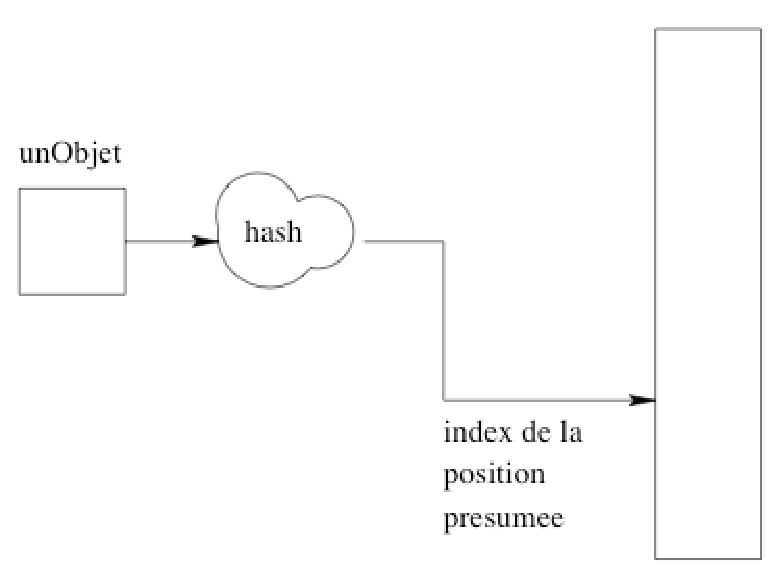
\includegraphics[width=8cm]{hash1}
%\caption{L'objet est hach\'e et on obtient un index dans la table}
%\label{fig:hash1}
%\end{center}
%\end{figure}

%\item L'index pr\'esum\'e ayant \'et\'e produit, on acc\`ede \`a la table.
%Si la table ne contient rien (\ct{nil}), alors l'objet n'est pas dans la table.
%Sinon on compare l'objet cherch\'e et l'objet trouv\'e (\ct{a = b}).
%Voir figure \ref{fig:hash2}.

%S'il y a \'egalit\'e, on a trouv\'e l'objet\ldots

%\begin{figure}[hbtp]
%\begin{center} 
%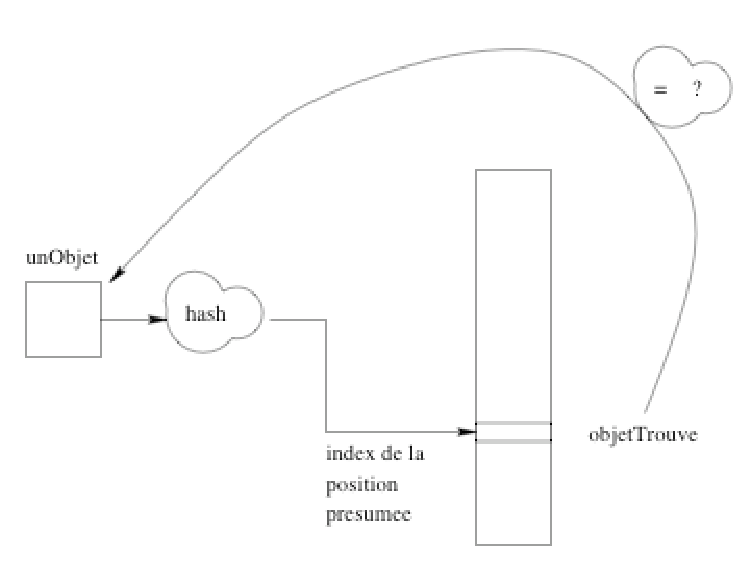
\includegraphics[width=8cm]{hash2} 
%\caption{On compare l'objet implant\'e dans la table et l'objet cherch\'e}
%\label{fig:hash2}
%\end{center} 
%\end{figure} 
%\newpage

%\item Sinon, on descend en s\'equence en cherchant soit \ct{nil}, soit
%l'\'egalit\'e (voir figure \ref{fig:hash3}).

%\begin{figure}[hbtp]
%\begin{center} 
%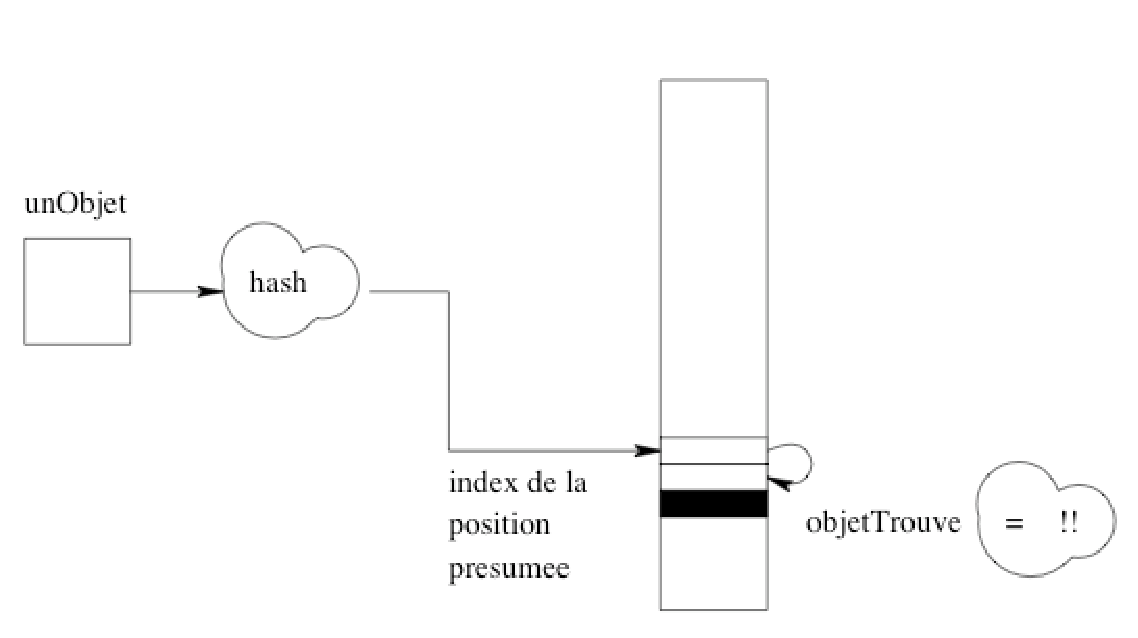
\includegraphics[width=8cm]{hash3} 
%\caption{Recherche en s\'equence}
%\label{fig:hash3}
%\end{center} 
%\end{figure} 
%\end{itemize}

%Les op\'erations d'insertion sont men\'ees de la m\^eme mani\`ere, il s'agit ici
%de trouver le premier index libre lors de la recherche en s\'equence. Lorsque
%la quantit\'e de collisions grandit (place libre de plus en plus petite),
%il est pr\'ef\'erable de reconstruire la table en doublant sa taille.

%
%Les suppressions requi\`erent une reconstruction au moins partielle de la table.

\ifx\wholebook\relax\else\end{document}\fi
